\documentclass[xcolor=dvipsnames,aspectratio=169]{beamer}
\usepackage[utf8]{inputenc}
\usetheme{Warsaw}
\usepackage{pgfpages}

% -----------------------------------------------------------------------------
% Notes toggle
% Compile with \def\NOTES{} before \input if you want notes-only output.
% -----------------------------------------------------------------------------
\newif\ifnotes
\ifdefined\NOTES\notestrue\fi
\ifnotes
  \setbeameroption{show only notes}
\else
  \setbeameroption{hide notes}
\fi

% -----------------------------------------------------------------------------
% Shared formatting
% -----------------------------------------------------------------------------
\setcounter{tocdepth}{2}

% =============================================================================
% Theme settings
% =============================================================================

% --- Core theme colors ---
\definecolor{ThemePrimary}{rgb}{0.0745, 0.1608, 0.2941}   % deep blue
\definecolor{ThemeSecondary}{rgb}{0.8667, 0.2039, 0.0118} % warm red/orange
\definecolor{ThemeAccent}{rgb}{0.1137, 0.3451, 0.6549}    % medium blue
\definecolor{ThemeLight}{rgb}{0.9725, 0.9804, 0.9882}     % near white
\definecolor{ThemeText}{rgb}{0.10, 0.10, 0.10}

% --- Optional extra palette ---
\definecolor{ThemeHighlight}{rgb}{0.9608, 0.5294, 0.1176}
\definecolor{ThemeSoftBlue}{rgb}{0.0000, 0.6235, 0.8314}
\definecolor{ThemeSoftNavy}{rgb}{0.1176, 0.2196, 0.4667}

% =============================================================================
% Beamer color settings
% =============================================================================

\setbeamercolor{palette primary}{bg=ThemePrimary,fg=ThemeLight}
\setbeamercolor{structure}{fg=ThemePrimary}
\setbeamercolor{section in toc}{fg=ThemePrimary}
\setbeamercolor{frametitle}{bg=ThemeSecondary,fg=ThemeLight}
\setbeamercolor{frametitle right}{bg=ThemePrimary}
\setbeamercolor{titlelike}{bg=ThemeSecondary,fg=ThemeLight}

% Optional tweaks you can enable later if desired:
% \setbeamercolor{block title}{bg=ThemePrimary,fg=ThemeLight}
% \setbeamercolor{block body}{bg=ThemeLight,fg=ThemeText}
% \setbeamercolor{section in head/foot}{bg=ThemeSoftNavy,fg=ThemeLight}
% \setbeamercolor{subsection in head/foot}{bg=ThemePrimary,fg=ThemeLight}

% =============================================================================
% Footline with page numbers
% =============================================================================

\defbeamertemplate*{footline}{shadow theme}{
    \leavevmode
    \hbox{%
        \begin{beamercolorbox}[
            wd=.5\paperwidth,
            ht=2.5ex,
            dp=1.125ex,
            leftskip=.3cm plus1fil,
            rightskip=.3cm
        ]{author in head/foot}
            \usebeamerfont{author in head/foot}\hfill\insertshortauthor
        \end{beamercolorbox}%
        \hskip0pt%
        \begin{beamercolorbox}[
            wd=.5\paperwidth,
            ht=2.5ex,
            dp=1.125ex,
            leftskip=.3cm,
            rightskip=.3cm plus1fil
        ]{title in head/foot}
            \usebeamerfont{title in head/foot}%
            \insertshorttitle\hfill\insertframenumber\,/\,\inserttotalframenumber
        \end{beamercolorbox}%
    }
    \vskip0pt
}

% =============================================================================
% Headline with current section / subsection
% =============================================================================

\setbeamertemplate{headline}{%
  \leavevmode
  \hbox{%
    \begin{beamercolorbox}[
        wd=.5\paperwidth,
        ht=2.1ex,
        dp=0.7ex,
        leftskip=0.3cm
    ]{section in head/foot}
      \usebeamerfont{section in head/foot}\insertsectionhead
    \end{beamercolorbox}%
    \begin{beamercolorbox}[
        wd=.5\paperwidth,
        ht=2.1ex,
        dp=0.7ex,
        rightskip=0.3cm
    ]{subsection in head/foot}
      \usebeamerfont{subsection in head/foot}\hfill\insertsubsectionhead
    \end{beamercolorbox}%
  }%
}

% =============================================================================
% Automatic outline slides
% =============================================================================

\AtBeginSection[]{
    \begin{frame}{Outline}
        \tableofcontents[currentsection]
    \end{frame}
}

\AtBeginSubsection[]{
    \begin{frame}{Outline}
        \tableofcontents[currentsection,currentsubsection]
    \end{frame}
}

% =============================================================================
% Figure / table packages
% =============================================================================

\usepackage{graphicx}   % figures
\usepackage{float}      % figure/table placement
\usepackage{rotating}   % rotated figures/tables
\usepackage{caption}    % captions
\usepackage{subcaption} % subfigures
\usepackage{makecell}   % table formatting
\usepackage{longtable}  % multipage tables
\usepackage{array}      % custom columns
\usepackage{tabularx}   % flexible-width tables
\usepackage{booktabs}   % professional tables

\newcolumntype{L}{>{\raggedright\arraybackslash}m{4cm}}
\newcolumntype{R}[1]{>{\raggedright\arraybackslash\hspace{0pt}\vspace{-0.25cm}}p{#1}}

% =============================================================================
% Math packages
% =============================================================================

\usepackage{amsfonts}
\usepackage{mathrsfs}
\usepackage{amsmath}
\usepackage{amssymb}
\usepackage{amsthm}
\usepackage{mathtools}
\usepackage{steinmetz}

% =============================================================================
% Chemistry / units
% =============================================================================

\usepackage[version=4]{mhchem}
\usepackage{chemformula}

\usepackage{siunitx}
\sisetup{locale = DE}
\sisetup{output-decimal-marker = {.}}

% =============================================================================
% Code / URL / verbatim
% =============================================================================

\usepackage{listings}
\usepackage{url}
\usepackage{verbatim}

% =============================================================================
% End of format file
% =============================================================================


% -----------------------------------------------------------------------------
% Presentation metadata
% Update these for each new talk.
% -----------------------------------------------------------------------------
\newcommand{\TalkTitle}{Computer Vision}
\newcommand{\TalkSubtitle}{Object Recognition}
\newcommand{\TalkAuthor}{Soo Min Kimm}
\newcommand{\TalkInstitute}{}
\newcommand{\TalkDate}{21/10/25}

\title{\TalkTitle}
\subtitle{\TalkSubtitle}
\author{\TalkAuthor}
\institute{\TalkInstitute}
\date{\TalkDate}

\begin{document}
    \begin{frame}
        \titlepage
    \end{frame}
    
    \begin{frame}{Outline}
        \tableofcontents
    \end{frame}

    \section{Computer Vision (CV)}
        \begin{frame}{Object Recognition}
            \begin{figure}
                \centering
                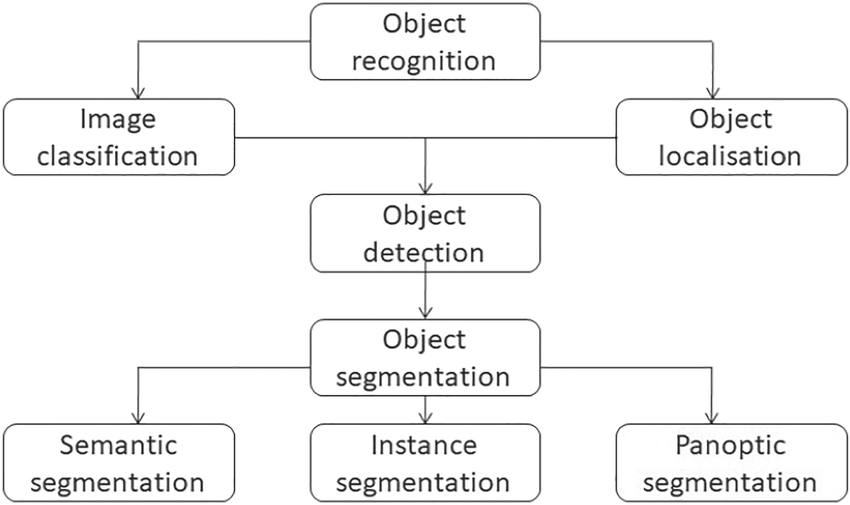
\includegraphics[width=0.6\linewidth]{figure/obj_recog.png}
                \caption{Overview of object recognition. Image from Brahmi \& Jdey (2023) - Automatic tooth instance segmentation and identification from panoramic X-Ray images using deep CNN.}
                \label{fig:obj_recog}
            \end{figure}
        \end{frame}

        \begin{frame}{Example}
            \begin{figure}
                \centering
                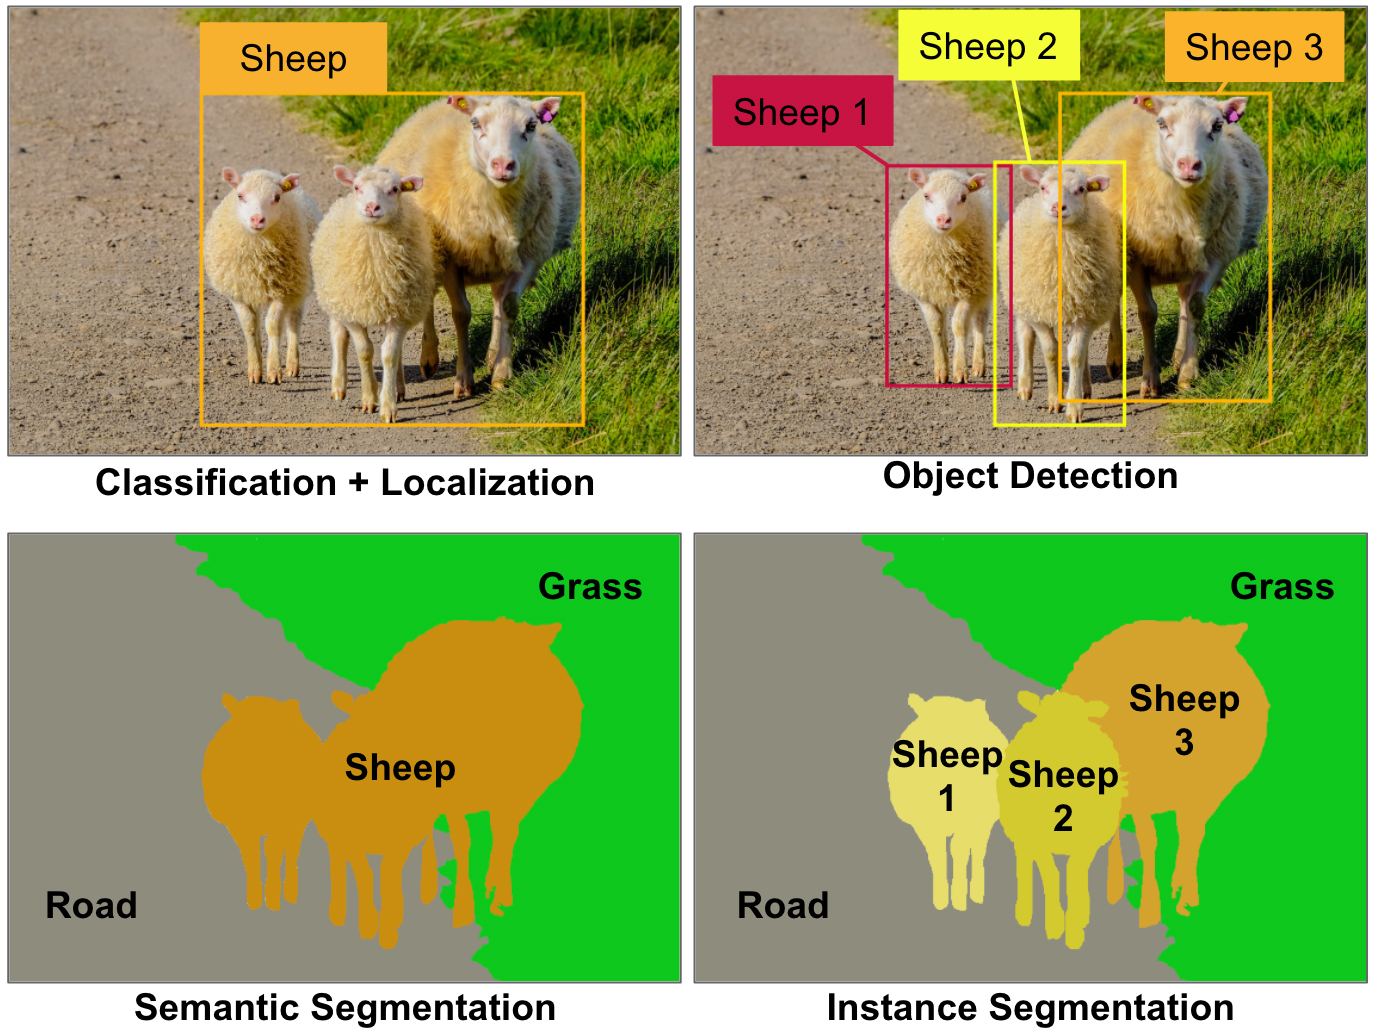
\includegraphics[width=0.5\linewidth]{figure/eg_obj_recog.png}
                \caption{Example of object recognition. Image from \url{https://www.oreilly.com/content/introducing-capsule-networks/?cmp=tw-data-na-article-ainy18_thea}}
                \label{fig:eg_obj_recog}
            \end{figure}
        \end{frame}

        \begin{frame}{Pipeline}
            \begin{figure}
                \centering
                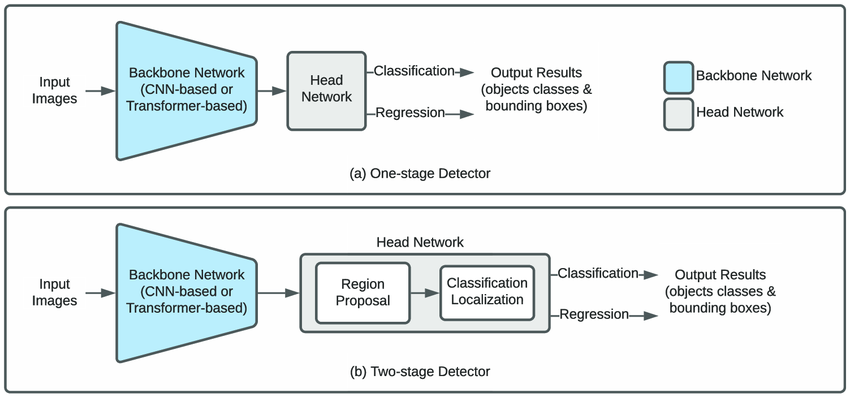
\includegraphics[width=0.8\linewidth]{figure/obj_detect.png}
                \caption{Pipeline of object detection. Image from Kang et al. (2022) - A Survey of Deep Learning-Based Object Detection Methods and Datasets for Overhead Imagery.}
                \label{fig:obj_detect}
            \end{figure}
        \end{frame}

        \begin{frame}{Evaluation Metrics}
            \begin{columns}[T]
                \begin{column}{0.48\textwidth}
                    \begin{block}{Intersection over Union (IoU)}
                        \begin{figure}
                            \centering
                            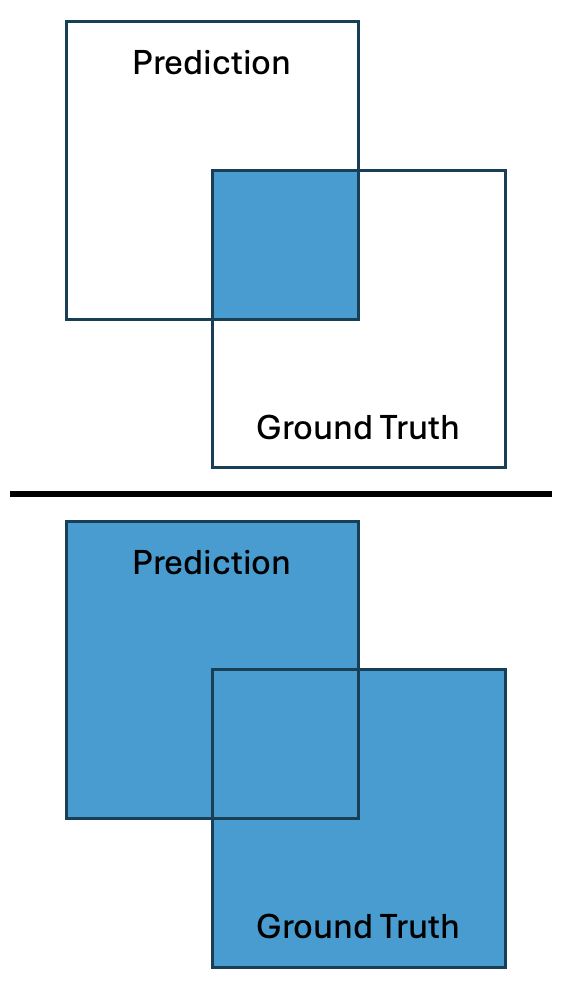
\includegraphics[width=0.4\linewidth]{figure/IoU.png}
                            \caption{$\mathrm{IoU} = \frac{X \cap Y}{X \cup Y}.$}
                            \label{fig:iou}
                        \end{figure}
                    \end{block}
                \end{column}
        
                \begin{column}{0.48\textwidth}
                    \begin{block}{Mean Average Precision (mAP)}
                        \begin{figure}
                            \centering
                            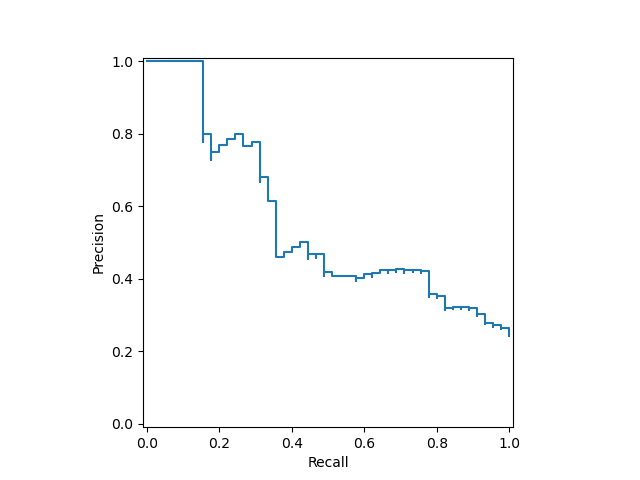
\includegraphics[width=0.7\linewidth]{figure/pr_curve.png}
                            \caption{$\mathrm{mAP} = \frac{1}{N} \sum_{k = 1}^{N} \mathrm{AP}_{i}$.}
                            \label{fig:pr_curve}
                        \end{figure}
                    \end{block}
                \end{column}
            \end{columns}
        \end{frame}

    \section{Backbone / Feature Extractor}
        \begin{frame}{Inductive Bias}
            A learning algorithm seeks a hypothesis $h \in \mathcal{H}$ that maps input $x$ to outputs $y$. \\
            Given training examples $D = \{ (x_{i}, y_{i}) \}$, there are typically infinitely many $h$ that can fit $D$. \\

            \begin{table}[h]
                \tiny
                \centering
                \renewcommand{\arraystretch}{1.4}
                \begin{tabular}{|l|p{5cm}|p{5cm}|}
                    \hline
                    \textbf{Type} & \textbf{Description} & \textbf{Example in Models} \\
                    \hline
                    \textbf{Architectural Bias} & 
                    Structure or connectivity built into the model. &
                    CNN’s local kernels, RNN’s recurrence, Transformer’s self-attention. \\
                    \hline
                    \textbf{Regularization Bias} & 
                    Added terms in the loss that prefer certain solutions. &
                    Weight decay, dropout, early stopping. \\
                    \hline
                    \textbf{Optimization Bias} & 
                    The way the model is trained can favor particular minima. &
                    SGD tends to find flatter minima (better generalization). \\
                    \hline
                    \textbf{Data Bias} & 
                    Augmentations or preprocessing that shape how data are “seen.” &
                    Rotations, flips, normalization. \\
                    \hline
                    \textbf{Prior Distribution Bias} & 
                    In Bayesian learning, priors encode assumptions about parameters. &
                    Gaussian prior in Bayesian linear regression. \\
                    \hline
                \end{tabular}
                \caption{Types of inductive bias.}
            \end{table}
        \end{frame}

        \begin{frame}{Receptive Field}
            For a unit at layer $L$ and spatial position $(i, j)$, the (theoretical) receptive field is the set of input pixels whose values can possibly affect that unit, given the network's filters, strides, dilations, and paddings.
    
            \begin{itemize}
                \item Theoretical RF: The Maximal geometric region implied by the architecture.
                \item Effective RF: The actual influence distribution within that region when the networks is trained—typically strongest at the centre and decaying outward. 
            \end{itemize}
        \end{frame}
    
        \subsection{Convolutional Neural Network (CNN)}
            \begin{frame}{Architecture}
                \begin{figure}
                    \centering
                    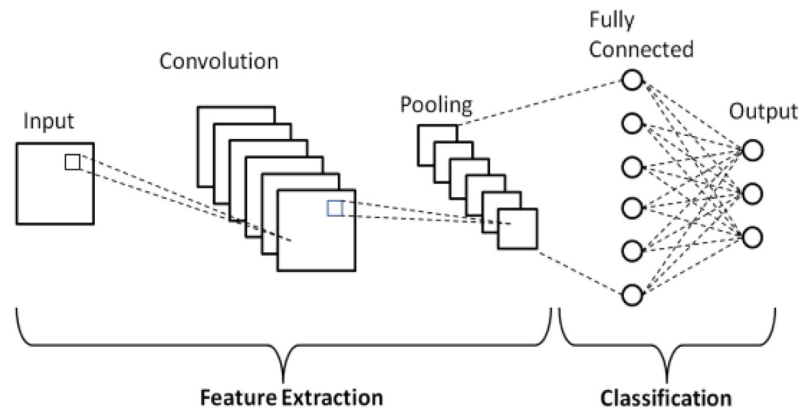
\includegraphics[width=0.7\linewidth]{figure/cnn.png}
                    \caption{CNN. Image from Phung \& Rhee (2018) - A Deep Learning Approach for Classification of Cloud Image Patches on Small Datasets.}
                    \label{fig:cnn}
                \end{figure}
            \end{frame}
    
            \begin{frame}{Definition}
                \footnotesize
                \begin{block}{Kernel}
                    Small learnable filter that extracts local patterns.
                \end{block}

                \begin{block}{Padding}
                    Adding zeros around the input to preserve spatial dimensions.
                \end{block}
    
                \begin{block}{Dilation}
                    Spacing elements in the kernel to enlarge receptive fields w/o more parameters.
                \end{block}
    
                \begin{block}{Stride}
                    Step size when sliding kernel that controls downsampling.
                \end{block}

                \begin{block}{Feature (Activation) Map}
                     The output tensor of a layer showing where and how strongly learned patterns appear. \\
                     Early feature maps: Edges, blobs, textures. \\
                     Deep feature maps: Object parts, semantics. 
                \end{block}
            \end{frame}

            \begin{frame}{Convolution}
                \begin{figure}
                    \centering
                    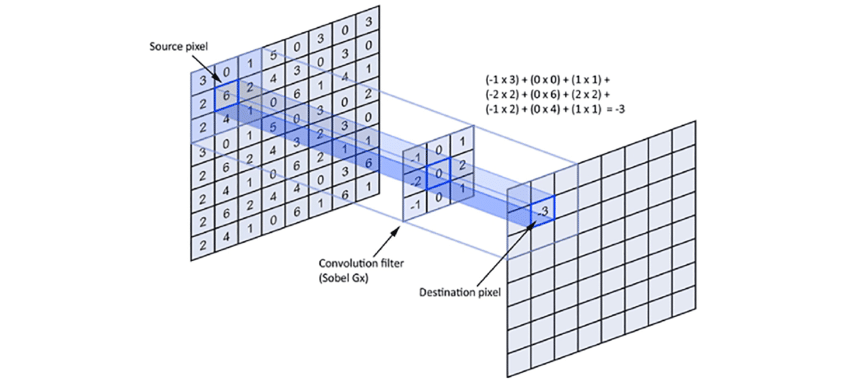
\includegraphics[width=0.7\linewidth]{figure/convolution.png}
                    \caption{Convolution. Image from Almryad \& Kutuku (2020) - Automatic Identification for Field Butterflies by CNN}
                    \label{fig:conv}
                \end{figure}
            \end{frame}
            
            \begin{frame}{Pooling}
                \begin{figure}
                    \centering
                    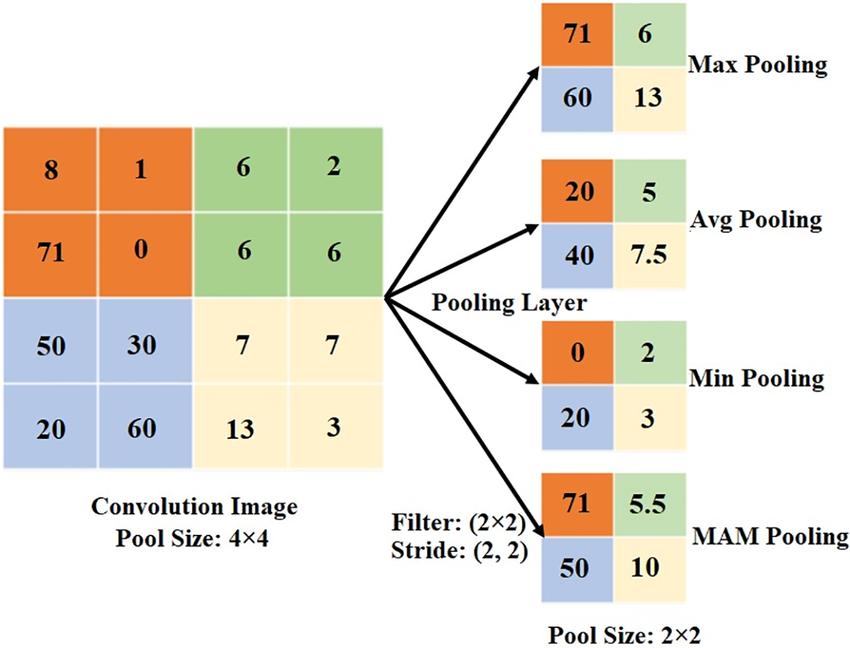
\includegraphics[width=0.5\linewidth]{figure/pooling.png}
                    \caption{Pooling. Image from Akgül (2024) - A Pooling Method Developed for Use in Convolutional Neural Networks.}
                    \label{fig:pooling}
                \end{figure}
            \end{frame}

            \subsubsection{Visual Geometry Group (VGG)}
                \begin{frame}{VGG: Architecture}
                    \begin{figure}
                        \centering
                        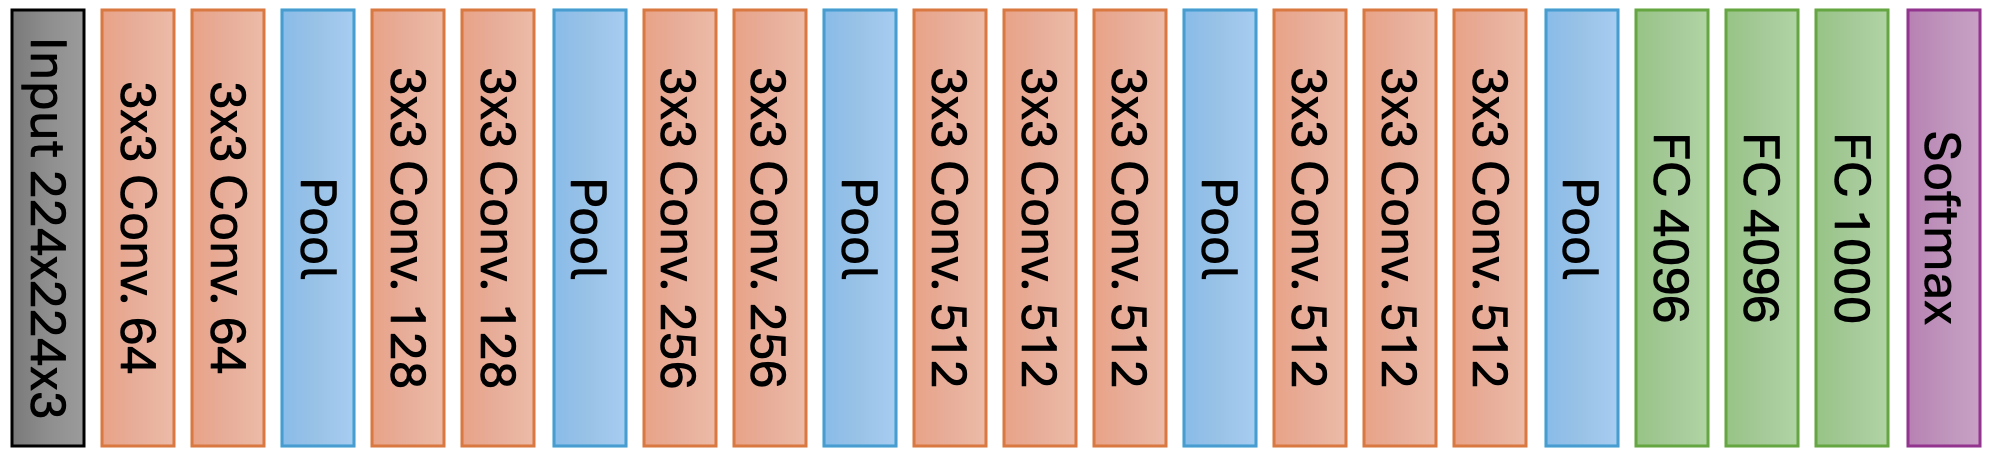
\includegraphics[width=1\linewidth]{figure/vgg.png}
                        \caption{VGG.}
                        \label{fig:vgg}
                    \end{figure}
                \end{frame}
                
            \subsubsection{Inception}
                \begin{frame}{Inception: Architecture}
                    \begin{figure}
                        \centering
                        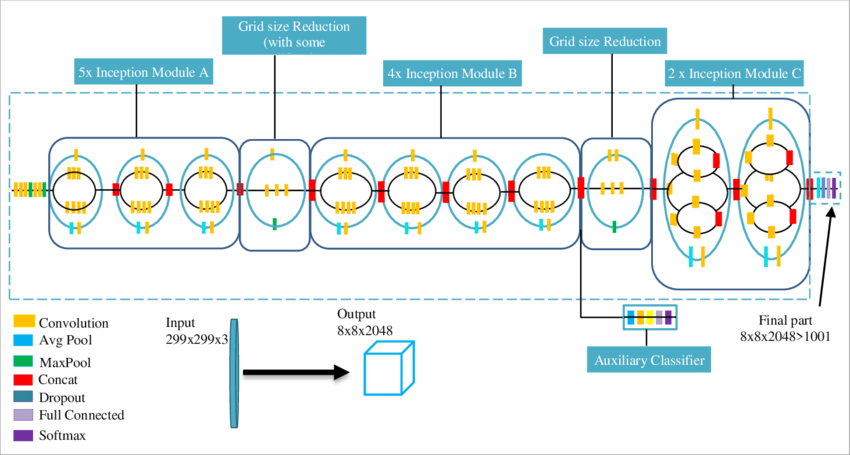
\includegraphics[width=0.75\linewidth]{figure/inception.png}
                        \caption{Inception. Image from Iparraguirre-Villanueva (2022) - Convolutional Neural Networks with Transfer Learning for Pneumonia Detection.}
                        \label{fig:inception}
                    \end{figure}
                \end{frame}

                \begin{frame}{VGG: $1 \times 1$ Convolution}
                    \begin{figure}
                        \centering
                        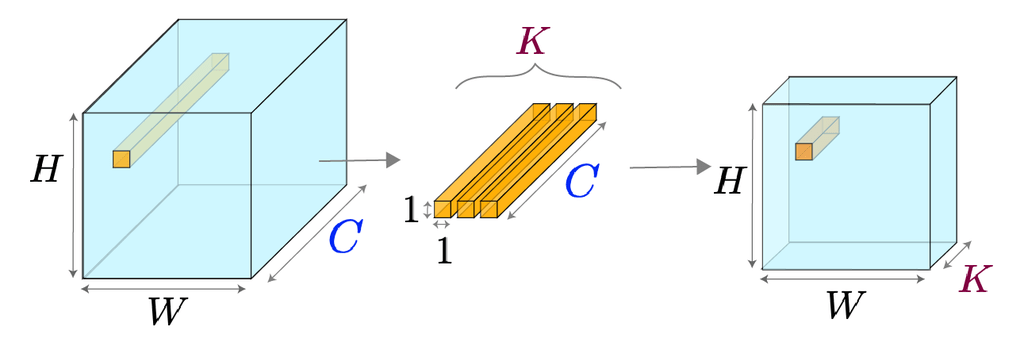
\includegraphics[width=0.6\linewidth]{figure/1x1_conv.png}
                        \caption{$1 \times 1$ convolution. Image from \url{https://cvml-expertguide.net/terms/dl/layers/convolution-layer/1x1-convolution/}.}
                        \label{fig:1x1_conv}
                    \end{figure}

                    \begin{itemize}
                        \item Combine information from different channels at the same spatial location
                        \item Reduce channel dimension
                    \end{itemize}
                \end{frame}
                
            \subsubsection{Residual Network (ResNet)}
                \begin{frame}{ResNet: Architecture}
                    \begin{figure}
                        \centering
                        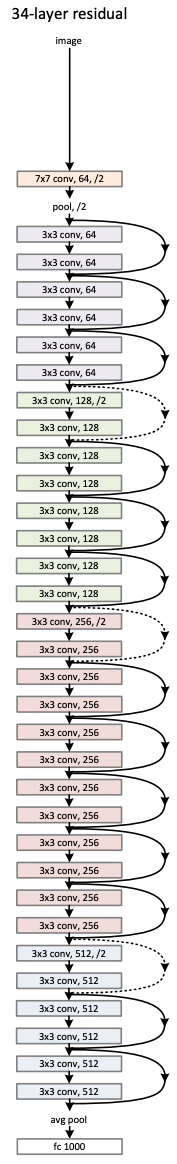
\includegraphics[width=0.15\linewidth, angle=270]{figure/resnet.png}
                        \caption{ResNet. Image from He et al. (2015) - Deep Residual Learning for Image Recognition.}
                        \label{fig:resnet}
                    \end{figure}
                \end{frame}

                \begin{frame}{ResNet: Residual Connection}
                    \begin{figure}
                        \centering
                        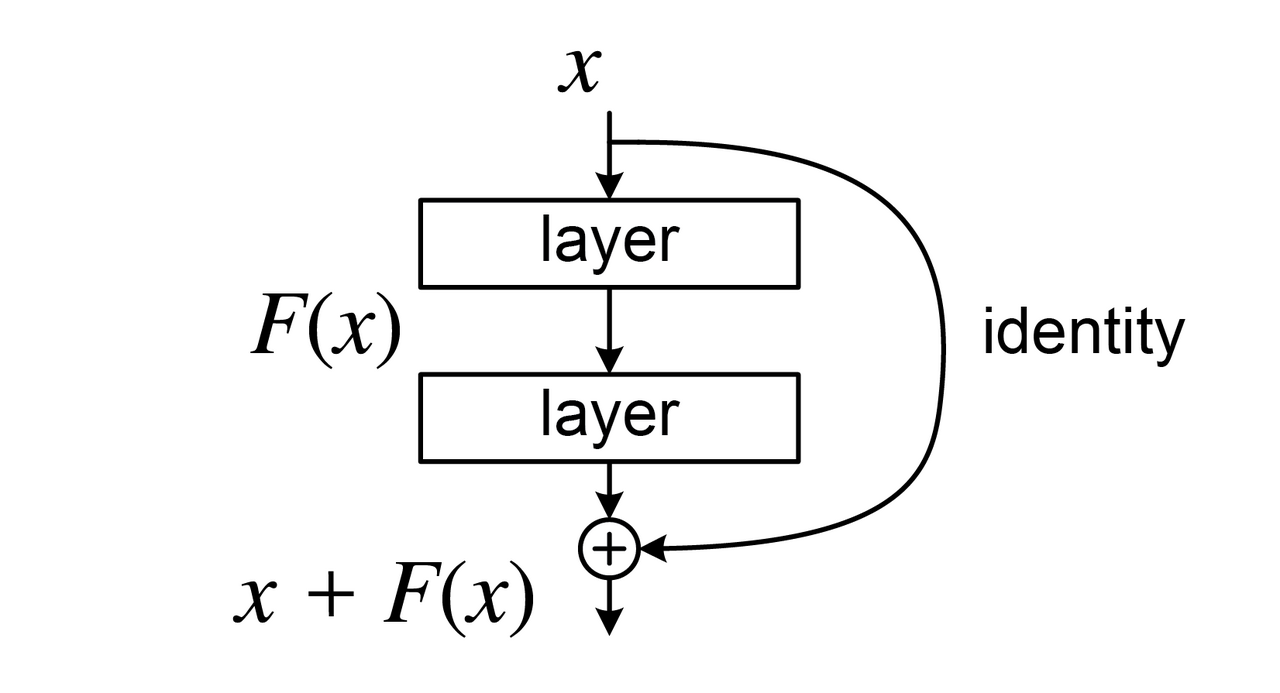
\includegraphics[width=0.4\linewidth]{figure/residual_connection.png}
                        \caption{Residual connection. Image from \url{https://www.wikipedia.com/en/articles/Residual_neural_network}.}
                        \label{fig:residual_connection}
                    \end{figure}

                    \begin{itemize}
                        \item Stable training by preserving gradient flow
                    \end{itemize}
                \end{frame}
    
        \subsection{Vision Transformer (ViT)}
            \begin{frame}{Architecture}
                \begin{figure}
                    \centering
                    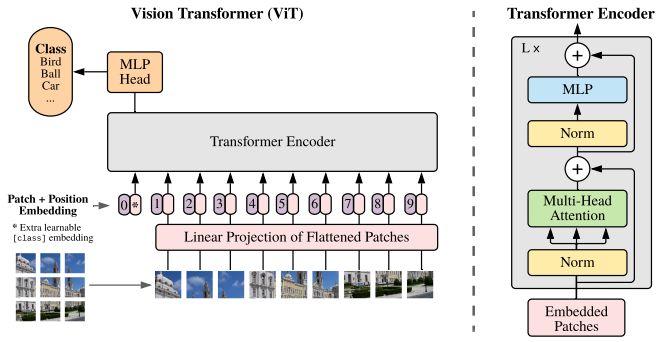
\includegraphics[width=0.5\linewidth]{figure/vit.png}
                    \caption{ViT. Image from Dosovitskiy et al. (2020) - An Image is Worth 16x16 Words.}
                    \label{fig:placeholder}
                \end{figure}

                \begin{itemize}
                    \item Class token summarises the entire sequence
                \end{itemize}
            \end{frame}

            \subsubsection{Data Efficient Image Transformer (DeiT)}
                \begin{frame}{DeiT: Architecture}
                    \begin{figure}
                        \centering
                        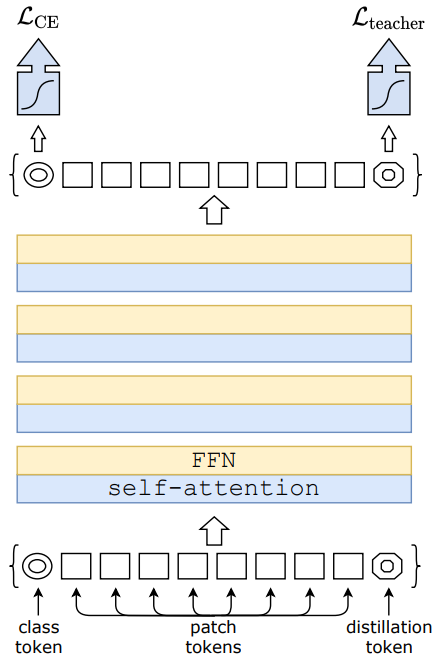
\includegraphics[width=0.2\linewidth]{figure/deit.png}
                        \caption{DeiT. Image from Touvron et al. (2020) - Training Data-Efficient Image Transformers \& Distillation through Attention.}
                        \label{fig:deit}
                    \end{figure}

                    \begin{itemize}
                        \item Class token learns from ground truth labels
                        \item Distillation token learns from teacher's outputs
                    \end{itemize}
                \end{frame}
            
                \begin{frame}{DeiT: Knowledge Distillation}
                    DeiT is trained as following:
                    
                    \begin{enumerate}
                        \item Train the CNN teacher and freeze the parameters once trained.
                        \item Train the ViT student to learn from the ground truth and the teacher's predictions.
                    \end{enumerate}

                    Loss is given as following:
                    
                    \begin{itemize}
                        \item Soft distillation: $\mathcal{L} = (1 - \lambda) \mathcal{L}_{\mathrm{CE}} (\psi (Z_{s}), y) + \lambda \tau^{2} \mathcal{L}_{\mathrm{KL}} (\psi (\frac{Z_{s}}{\tau}), \psi (\frac{Z_{t}}{\tau}))$
                        \item Hard distillation: $\mathcal{L} = \frac{1}{2} \mathcal{L}_{\mathrm{CE}} (\psi (Z_{s}), y) + \frac{1}{2} \mathcal{L}_{\mathrm{CE}} (\psi (Z_{t}), y_{t})$
                    \end{itemize}

                    where $Z_{t}, Z_{s}$ are logits of teacher and student models respectively, $\tau$ is the distillation temperature, $\lambda$ is the coefficient balancing $\mathcal{L}_{\mathrm{KL}}$, $y_{t} = \arg \max_{c} Z_{t} (c)$, and $\psi$ is the softmax function.
                \end{frame}
                
            \subsubsection{Shifted Windows (Swin) Transformer}
                \begin{frame}{Swin Transformer: Architecture}
                    \begin{figure}
                        \centering
                        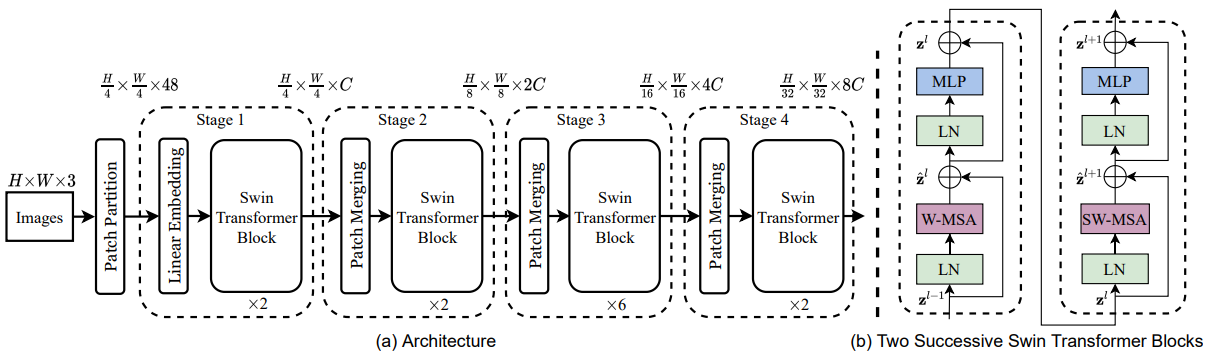
\includegraphics[width=0.9\linewidth]{figure/swin.png}
                        \caption{Swin Transformer. Image from Liu et al. (2021) - Swin Transformer.}
                        \label{fig:swin}
                    \end{figure}
                \end{frame}

                \begin{frame}{Swin Transformer: Shifted Window}
                    \begin{figure}[h]
                        \begin{subfigure}{0.45\textwidth}
                            \centering
                            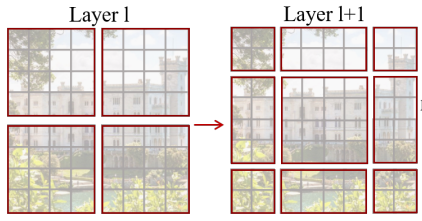
\includegraphics[width=1\linewidth]{figure/shifted_window.png}
                            \caption{Shifted window}
                            \label{fig:shifted_window}
                        \end{subfigure}
                        \begin{subfigure}{0.45\textwidth}
                            \centering
                            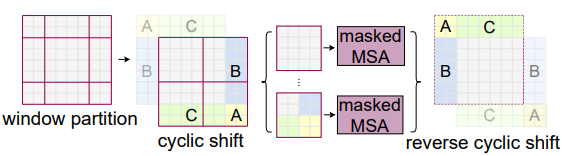
\includegraphics[width=1\linewidth]{figure/shifted_patches.png}
                            \caption{Shifted patches}
                            \label{fig:shifted_patches}
                        \end{subfigure}
                        \caption{Shifted window partitioning. Image from Liu et al. (2021) - Swin Transformer.}
                        \label{fig:shifted_window_partitioning}
                    \end{figure}
                \end{frame}

                \begin{frame}{Swin Transformer: Hierarchy}
                    \begin{figure}
                        \centering
                        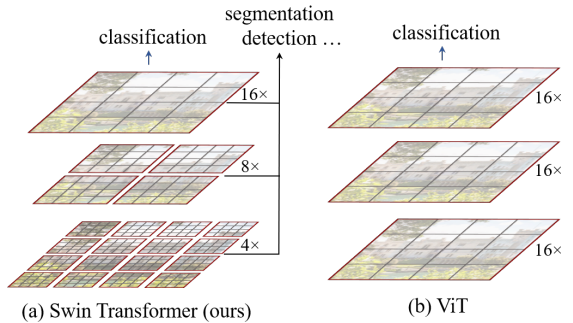
\includegraphics[width=0.5\linewidth]{figure/swin_hierarchy.png}
                        \caption{Hierarchy of Swin Transformer. Image from Liu et al. (2021) - Swin Transformer.}
                        \label{fig:swin_hierarchy}
                    \end{figure}
                \end{frame}
                
    \section{Detector}
        \subsection{R-CNN}
            \begin{frame}{Pipeline}
                \begin{figure}
					\centering
					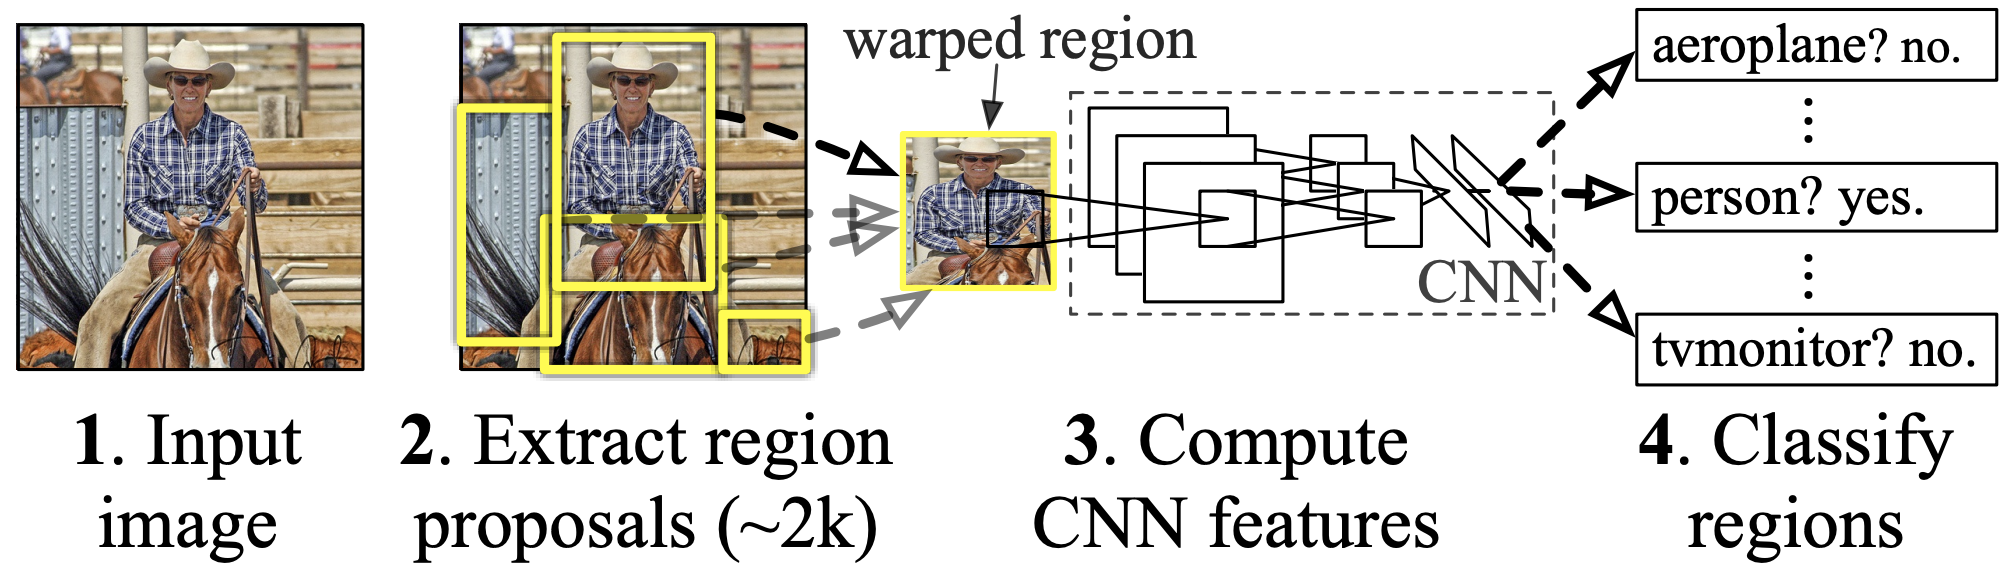
\includegraphics[width=0.8\linewidth]{figure/r_cnn.png}
					\caption{R-CNN. Image from Girshick et al. (2014) - Rich Feature Hierarchies for Accurate Object Detection and Semantic Segmentation.}
					\label{fig:r_cnn}
				\end{figure}
            \end{frame}

            \begin{frame}{Selective Search}
                \begin{figure}
					\centering
					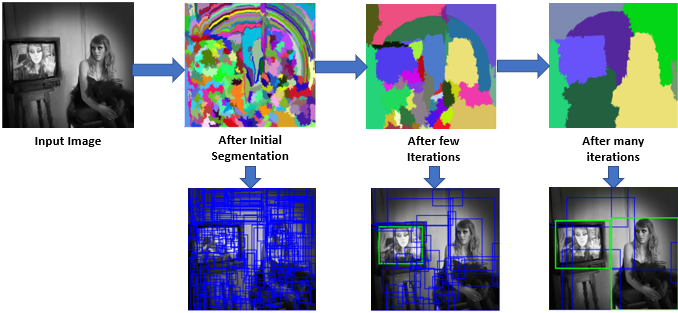
\includegraphics[width=0.8\linewidth]{figure/selective_search.png}
					\caption{Selective search algorithm. Image from Uijlings et al. (2013) - Selective Search for Object Recognition.}
					\label{fig:selective_search}
				\end{figure}
            \end{frame}

            \begin{frame}{Hard Negative Mining}
                
            \end{frame}

            \begin{frame}{Non-Maximum Suppression}
                
            \end{frame}

            \begin{frame}{Contributions \& Limitations}
                
            \end{frame}

        \subsection{Fast R-CNN}
            \begin{frame}{Pipeline}
                
            \end{frame}

            \begin{frame}{RoI Pooling}
                
            \end{frame}

            \begin{frame}{Truncated SVD}
                
            \end{frame}

            \begin{frame}{Contributions \& Limitations}
                
            \end{frame}

        \subsection{Faster R-CNN}
            \begin{frame}{Pipeline}
                
            \end{frame}

            \begin{frame}{Region Proposal Network (RPN)}
                
            \end{frame}

            \begin{frame}{Contributions \& Limitations}
                
            \end{frame}

        \subsection{YOLO}
            \begin{frame}{Pipeline}
                
            \end{frame}

            \begin{frame}{Contributions \& Limitations}
                
            \end{frame}

        \subsection{SSD}
            \begin{frame}{Pipeline}
                
            \end{frame}

            \begin{frame}{Contributions \& Limitations}
                
            \end{frame}

        \subsection{DETR}
            \begin{frame}{Pipeline}
                
            \end{frame}

            \begin{frame}{Hungarian Matching Algorithm}
                
            \end{frame}

            \begin{frame}{Contributions \& Limitations}
                
            \end{frame}

        \subsection{Deformable DETR}
            \begin{frame}{Pipeline}
                
            \end{frame}

            \begin{frame}{Deformable Convolution}
                
            \end{frame}

            \begin{frame}{Deformable Attention}
                
            \end{frame}

            \begin{frame}{Contributions \& Limitations}
                
            \end{frame}

        \subsection{DINO}
            \begin{frame}{Pipeline}
                
            \end{frame}

            \begin{frame}{Self-Supervised Knowledge Distillation}
                
            \end{frame}

            \begin{frame}{Contributions \& Limitations}
                
            \end{frame}

    \section{Summary}
        \begin{frame}{Summary 1}
            \begin{table}
                \tiny
                \setlength{\tabcolsep}{3pt}
                \renewcommand{\arraystretch}{1.35}
                \begin{tabular}{|l|c|c|c|c|}
                    \hline
                    \textbf{Model} & \textbf{Stage} & \textbf{Proposals / Anchors} & \textbf{NMS} & \textbf{Matching} \\
                    \hline
                    R-CNN & 2-stage & Selective Search (2k) & Yes & IoU-based \\
                    \hline
                    Fast R-CNN & 2-stage & Selective Search (external) & Yes & IoU-based \\
                    \hline
                    Faster R-CNN & 2-stage & RPN (anchor-based) & Yes & IoU / anchor assign \\
                    \hline
                    YOLO (v1) & 1-stage & Grid-based boxes (anchor-free-ish) & Yes & Grid responsibility \\
                    \hline
                    SSD & 1-stage & Default boxes (multi-scale anchors) & Yes & IoU / anchor assign \\
                    \hline
                    DETR & Set-based & None (no anchors) & No & Hungarian (bipartite) \\
                    \hline
                    Deformable DETR & Set-based & None & No & Hungarian (bipartite) \\
                    \hline
                    DINO & Set-based & None & No & Hungarian (bipartite) \\
                    \hline
                \end{tabular}
                \caption{Properties of detectors.}
            \end{table}
        \end{frame}    

    \begin{frame}{Summary 2}
        \begin{table}
            \tiny
            \setlength{\tabcolsep}{3pt}
            \renewcommand{\arraystretch}{1.35}
            \begin{tabular}{|l|p{5.5cm}|p{5.5cm}|}
                \hline
                \textbf{Model} & \textbf{Key Ideas / Strengths} & \textbf{Limitations / Notes} \\
                \hline
                R-CNN & Deep features for detection; strong accuracy for its time. & Very slow (per-RoI CNN); no shared conv features; multi-step pipeline. \\
                \hline
                Fast R-CNN & Single CNN for image; RoI Pooling; joint classification \& regression. & Still depends on external proposals; not real-time. \\
                \hline
                Faster R-CNN & Region Proposal Network (RPN); shared conv features; end-to-end. & Requires anchor tuning; slower than one-stage. \\
                \hline
                YOLO (v1) & Real-time, single forward pass; simple end-to-end training. & Struggles with small/overlapping objects; coarse grid. \\
                \hline
                SSD & Multi-scale feature maps; fast and lightweight. & Fixed anchors; limited context; requires tuning. \\
                \hline
                DETR & End-to-end set prediction; no anchors/NMS; simple loss. & Slow convergence; weak for small objects. \\
                \hline
                Deformable DETR & Deformable multi-scale attention; faster convergence; sparse sampling. & Complex implementation; heavy computation. \\
                \hline
                DINO & Self-distillation; denoising queries; strong accuracy. & Transformer latency; careful training recipe needed. \\
                \hline
            \end{tabular}
            \caption{Overview of detectors.}
        \end{table}
    \end{frame}
\end{document}